\textbf{RND normaliser (all eight tasks).} The bottom block of Table~\ref{tab:main} compares the guarded normaliser of (\ref{eq:rnd}) with its variants; Table~\ref{tab:diag} gives bonus diagnostics over the 40 runs of each variant.


\begin{table}[!tb]\centering\caption{Bonus diagnostics of the RND variants over 40 runs each (8 tasks $\times$ 5 seeds). Spike: $b>10^4$ within the first 100 steps. ``found'': runs that found the reward. Median $b$: median over runs of the per-run median; max $b$ and max $|Q|$: maximum over runs; share of steps with $b>1$ (positive shaped reward): mean over runs.}\label{tab:diag}{\footnotesize\setlength{\tabcolsep}{2.7pt}\begin{tabular}{lrrrrr}
\hline
 & guarded & clip only & warm-up & v1 & no norm. \\
\hline
spike runs (of 40) & 0 & 0 & 0 & 20 & 0 \\
found, spike runs & -- & -- & -- & 1/20 & -- \\
found, other runs & 39/40 & 39/40 & 38/40 & 20/20 & 40/40 \\
median $b$ & \rhval{main/rnd-bonus/room_6/bonus_median/median} & \rhval{main/rnd-clip-only/room_6/bonus_median/median} & \rhval{main/rnd-warm-up-only/room_6/bonus_median/median} & \rhval{main/rnd-unguarded-normaliser-v1/room_6/bonus_median/median} & \rhval{main/no-bonus-normalisation-rnd_nonorm/room_6/bonus_median/median} \\
max $b$ & \rhval{main/rnd-bonus/room_6/bonus_max/max} & \rhval{main/rnd-clip-only/room_6/bonus_max/max} & \rhval{main/rnd-warm-up-only/room_4/bonus_max/max} & \rhval{main/rnd-unguarded-normaliser-v1/chain_20_tv/bonus_max/max} & \rhval{main/no-bonus-normalisation-rnd_nonorm/chain_20_tv/bonus_max/max} \\
share $b>1$ & \rhval{main/rnd-bonus/room_6/bonus_gt1_frac/mean} & \rhval{main/rnd-clip-only/room_6/bonus_gt1_frac/mean} & \rhval{main/rnd-warm-up-only/room_6/bonus_gt1_frac/mean} & \rhval{main/rnd-unguarded-normaliser-v1/room_6/bonus_gt1_frac/mean} & \rhval{main/no-bonus-normalisation-rnd_nonorm/room_6/bonus_gt1_frac/mean} \\
max $|Q|$ & \rhval{main/rnd-bonus/room_2/q_abs_max/max} & \rhval{main/rnd-clip-only/room_2/q_abs_max/max} & \rhval{main/rnd-warm-up-only/room_4/q_abs_max/max} & \rhval{main/rnd-unguarded-normaliser-v1/chain_10/q_abs_max/max} & \rhval{main/no-bonus-normalisation-rnd_nonorm/room_6/q_abs_max/max} \\
\hline
\end{tabular}
}\end{table}

\begin{figure}[!tb]\centering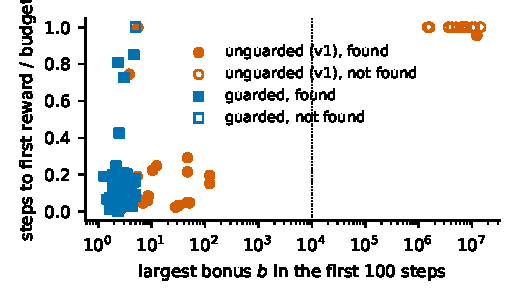
\includegraphics[width=0.92\columnwidth]{generated/spike_vs_steps.pdf}\caption{One point per run (8 tasks $\times$ 5 seeds): largest bonus in the first 100 steps against steps to first reward as a fraction of the budget, for the unguarded and the guarded normaliser. Dotted line: spike threshold $10^4$.}\label{fig:spike}\end{figure}

\emph{Failure case: the unguarded normaliser.} The first version of this study used $b=e/(\sigma_e+10^{-8})$ from the first step. When the first arrival observations coincide (the agent stays on the start cell or bumps into a wall) the errors are identical, because the predictor is first updated after eight transitions, so $\sigma_e=0$ and the bonus is $e\times10^{8}$. Table~\ref{tab:diag} shows the consequence: 20 of the 40 unguarded runs have such a spike, with bonuses up to $1.44\times10^{7}$ and Q-values up to $3.62\times10^{6}$, and only 1 of these 20 finds the reward (chain\_10, after 28656 of 30000 steps), whereas all 20 runs without a spike find it. Fig.~\ref{fig:spike} shows the two groups, separated by four orders of magnitude in the early bonus (the spike threshold of $10^4$ was set after seeing this gap). The intervention confirms the cause: with only the clip, or only the warm-up, no run has a spike and 39 and 38 of 40 runs find the reward. The failures of the unguarded variant in Table~\ref{tab:main} (for example only 2 of 5 seeds succeed on room\_4 and on room\_6) are therefore a numerical artefact of the normaliser and say nothing about the novelty signal.

\emph{Guarded variants.} Guarded, clip-only and warm-up-only RND behave alike (Table~\ref{tab:main}): each finds the reward in 38 or 39 of 40 runs, and their means differ less from each other than from the unguarded variant. Clip-only is the slowest of the three on the noise-free chains and on room\_4\_tv (for example 915, 6493 and 19682 steps on chain\_10, chain\_40 and room\_4\_tv against 525, 5242 and 15184 for the guarded method). The warm-up alone still lets the bonus reach 29, without visible harm. All three are slower than the penalty-only control on every task.

\emph{No normalisation.} The raw error never exceeds 0.44 and is never above the offset of 1 (share $b>1$: 0.000), so this variant is a step penalty of about $\beta$ with a small perturbation. Its means track the penalty-only control (for example 2620 against 2638 on chain\_40 and 29808 against 29105 on room\_6), with deviations in both directions: faster on chain\_10 (64 against 122) and room\_4\_tv (11439 against 13231), slower on room\_4 (13206 against 11921). It finds the reward in all 40 runs, but this shows that the raw error is too small to matter, not that the novelty signal works.

\emph{Why is normalised RND slower than no bonus?} The normalised bonus is close to zero most of the time (median 0.0005) and exceeds the offset on a share of 0.018 of the steps. Such positive shaped rewards make recently novel cells attractive to revisit, which may be what costs time; we did not isolate this.

\textbf{Clip $c$ (chain\_20, room\_4).} Table~\ref{tab:clip}: a tighter clip ($c=2$) gives lower means than $c=5$ on both tasks (1730 against 2146 and 15396 against 18435 steps), and $c=20$ is identical to no clip because the bonus never reached 20 after the warm-up on these tasks. All settings find the reward in every seed and all remain slower than the penalty-only control (618 and 11921 steps). The differences between clip values are of the order of one standard deviation and were not tested; the main result does not hinge on $c=5$.

\begin{table}[!tb]\centering\caption{Clip sweep for the RND bonus (warm-up 64): steps to first reward (mean $\pm$ std over 5 seeds) and share of clipped steps. Every setting finds the reward in all five seeds. $c=5$ is the main setting; ``none'' is the warm-up-only variant.}\label{tab:clip}{\footnotesize\begin{tabular}{lrrrr}
\hline
$c$ & chain\_20 steps & clipped & room\_4 steps & clipped \\
\hline
2 & 1730 $\pm$ 124 & 0.005 & 15396 $\pm$ 2996 & 0.005 \\
5 & 2146 $\pm$ 448 & 0.000 & 18435 $\pm$ 4082 & 0.001 \\
20 & 2051 $\pm$ 447 & 0.000 & 19474 $\pm$ 2608 & 0.000 \\
none & 2051 $\pm$ 447 & 0.000 & 19474 $\pm$ 2608 & 0.000 \\
\hline
\end{tabular}
}\end{table}

\textbf{Token cardinality $K$ (H4, room\_4\_tv).} Table~\ref{tab:K}: the TV share rises monotonically with $K$ for both systems that see the token, from $0.016$ to $0.029$ for RND and from $0.013$ to $0.027$ for the observation count (Welch $p<0.001$ between $K=1$ and $K=64$), while steps to first reward shows no systematic change ($p=0.406$ and $0.511$). At $K=1$ the observation count equals the state count by construction. \emph{H4 is supported for the time spent on the TV and not for the time to reward}: more tokens roughly double the TV share, but it stays below 0.03 and costs nothing measurable.

\begin{table}[!tb]\centering\caption{Sweep over the TV token cardinality $K$ on room\_4\_tv (mean $\pm$ std over 5 seeds): steps to first reward and TV share for RND and the observation count (Cnt). Last row: Welch $p$ between $K=1$ and $K=64$. $K=16$ is the main setting.}\label{tab:K}\resizebox{\columnwidth}{!}{\footnotesize\setlength{\tabcolsep}{3pt}\begin{tabular}{lrrrr}
\hline
$K$ & RND steps & RND TV & Cnt steps & Cnt TV \\
\hline
1 & 18383 $\pm$ 2341 & 0.016 $\pm$ 0.002 & 11476 $\pm$ 2146 & 0.013 $\pm$ 0.000 \\
4 & 17831 $\pm$ 1639 & 0.020 $\pm$ 0.001 & 12117 $\pm$ 1142 & 0.018 $\pm$ 0.001 \\
16 & 15184 $\pm$ 3604 & 0.025 $\pm$ 0.001 & 11142 $\pm$ 2646 & 0.023 $\pm$ 0.001 \\
64 & 19695 $\pm$ 2381 & 0.029 $\pm$ 0.002 & 12247 $\pm$ 1238 & 0.027 $\pm$ 0.000 \\
\hline
\end{tabular}
}\end{table}

\textbf{Bonus scale $\beta$ (room\_4).} For $\beta\in\{0.03,0.1,0.3,1\}$ steps to first reward is identical for the RND and the count bonus (\texttt{results/tables/sweep\_beta\_perconfig.md} in the repository), as the linearity argument of Section~\ref{sec:method} predicts; the sweep says nothing more about $\beta$.
